\subsection{Channels}

\frame{\tableofcontents[currentsubsection]}

\begin{frame}
  \frametitle{Number of Channels}
  \begin{itemize}
    \item WAV supports mono and stereo
    \item Stereo means that there are 2 separate wave functions
    \item The samples of both waves are interleaved
  \end{itemize}
  \begin{center}
    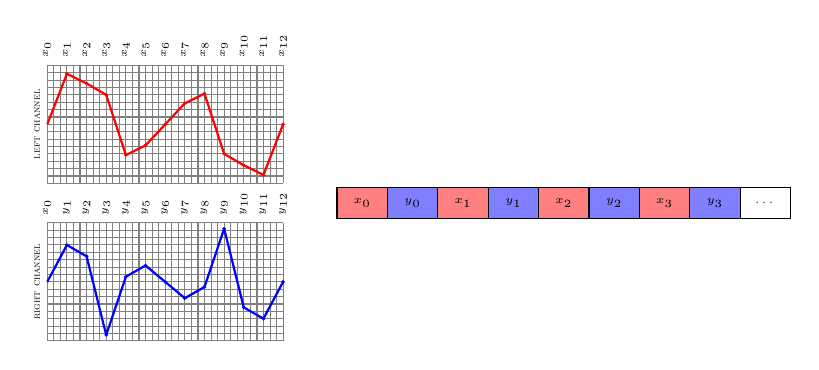
\begin{tikzpicture}[channel/.style={draw,font=\tiny,minimum height=5mm,minimum width=8mm},
                        channel 1/.style={channel,fill=red!50},
                        channel 2/.style={channel,fill=blue!50}]
      \begin{scope}[yshift=1cm,scale=.75,transform shape]
        \draw[thin,gray] (0,-1) grid[xstep=0.111cm,ystep=0.125cm] (4,1);
        \foreach[count=\i,
                 evaluate={0.7*sin(2*\x)+0.2*sin(5*\x)+0.3*sin(13*\x)} as \y,
                 remember=\y as \lasty (initially 0),
                 remember=\x as \lastx (initially 0)] \x in {30,60,...,360} {
          \draw[fill,red] (\x*0.0111,\y) circle [radius=0.02cm];
          \node[right,font=\tiny,rotate=90] at (\x*0.0111,1) {$x_{\i}$};
          \draw[thick,red] (\lastx*0.0111,\lasty) -- (\x*0.0111,\y);
        }
        \node[right,font=\tiny,rotate=90] at (0,1) {$x_0$};
        \node[rotate=90,anchor=south,font=\scshape\tiny] at (0,0) {left channel};
      \end{scope}
      \begin{scope}[yshift=-1cm,scale=.75,transform shape]
        \draw[thin,gray] (0,-1) grid[xstep=0.111cm,ystep=0.125cm] (4,1);
        \foreach[count=\i,
                 evaluate={0.6*sin(3*\x)+0.2*sin(2*\x)+0.3*sin(-17*\x)} as \y,
                 remember=\y as \lasty (initially 0),
                 remember=\x as \lastx (initially 0)] \x in {30,60,...,360} {
          \draw[fill,blue] (\x*0.0111,\y) circle [radius=0.02cm];
          \node[right,font=\tiny,rotate=90] at (\x*0.0111,1) {$y_{\i}$};
          \draw[thick,blue] (\lastx*0.0111,\lasty) -- (\x*0.0111,\y);
        }
        \node[right,font=\tiny,rotate=90] at (0,1) {$x_0$};
        \node[rotate=90,anchor=south,font=\scshape\tiny] at (0,0) {right channel};
      \end{scope}
      \begin{scope}[xshift=4cm,scale=.8,transform shape]
        \foreach \i in {0,...,3} {
          \node[channel 1] at (\i*0.8*2,0) {$x_{\i}$};
          \node[channel 2] at (\i*0.8*2+0.8,0) {$y_{\i}$};
        }
        \node[channel] at (8*0.8,0) {\dots};
      \end{scope}
    \end{tikzpicture}
  \end{center}
\end{frame}

\begin{frame}
  \frametitle{Dealing With Stereo Sound}
  \begin{center}
    \begin{tikzpicture}[milestone/.style={drop shadow,draw,fill=red!50,minimum height=7.5mm,minimum width=1cm,font=\tiny\scshape},
                        link/.style={-latex,thick},
                        arrow/.style={blue,ultra thick,-{Stealth[]}},
                        scale=.8,transform shape]
      \node[milestone] (uint8) at (0,0) {\texttt{Stream<uint8>}};
      \node[milestone] (int16) at ($ (uint8) + (2,1) $) {\texttt{Stream<int16>}};
      \node[milestone] (double) at ($ (uint8) + (4,0) $) {\texttt{Stream<double>}};
      \node[milestone] (double1) at ($ (double) + (3,1) $) {\texttt{Stream<double>}};
      \node[milestone] (double2) at ($ (double) + (3,-1) $) {\texttt{Stream<double>}};
      \node[milestone] (wave1) at ($ (double1) + (3,0) $) {\texttt{Wave}};
      \node[milestone] (wave2) at ($ (double2) + (3,0) $) {\texttt{Wave}};

      \coordinate (double top exit) at ($ (double.north) ! 0.5 ! (double.north east) $);
      \coordinate (double bottom exit) at ($ (double.south) ! 0.5 ! (double.south east) $);

      \draw[link] (uint8) |- (int16);
      \draw[link] (int16) -| (double);
      \draw[link] (uint8) -- (double);
      \draw[link] (double top exit) |- (double1);
      \draw[link] (double bottom exit) |- (double2);
      \draw[link] (double1) -- (wave1);
      \draw[link] (double2) -- (wave2);
    \end{tikzpicture}
  \end{center}
  \begin{itemize}
    \item In case of stereo sound, we need to split up the \texttt{Stream<double>} into two
    \item This way, we end up with one \texttt{Wave} per channel
  \end{itemize}
\end{frame}



%%% Local Variables:
%%% mode: latex
%%% TeX-master: "sound"
%%% End:
